\documentclass[letterpaper, 12pt, oneside]{book}
\usepackage[margin = 1in, includehead, footskip=0.25in]{geometry}
\usepackage{setspace}
\usepackage{caption}
\usepackage{subcaption}
\doublespacing
\usepackage{amsfonts}
\usepackage{amsmath}
\usepackage{amsthm}
\usepackage{tikz}
\usepackage{graphicx}
\usepackage{multirow}
\usepackage{booktabs}
\usepackage{tabularx}
\usepackage{longtable}
\usepackage{lscape}
\usepackage{import}
\usepackage[style=phys]{biblatex}
\newcommand{\dd}{\textrm{d}}
\bibliography{thesis_refs}
%\addbibresource{thesis_refs.bib}
\usepackage{lineno}
\linenumbers
\usepackage[pdfauthor={My Full Name},
    pdftitle={Title},
    hidelinks
]{hyperref}
\newtheorem{lemma}{Lemma}[section]
\theoremstyle{definition}
\newtheorem{definition}{Definition}[section]
\newtheorem{corolary}{Corolary}[section]
%\author{Skadi K Grossberndt}
%\title{Energy Correlators as a probe of the hard process in Run 24 $p-p$ collisions at $\sqrt{s}=200$ $GeV$ with the sPHENIX detector at RHIC}
%\affil{Graduate Center and Baruch College, CUNY}
\begin{document}
%\maketitle
\frontmatter
\begin{titlepage}

\begin{center}

~\vspace{2in}

\textsc{Energy Correlators as a probe of the hard process in Run 24 $p-p$ collisions at $\sqrt{s}=200$ $GeV$ with the sPHENIX detector at RHIC} \\[0.5in]
by \\[0.5in]
\textsc{Skadi Kurt Grossberndt} 

\vspace{\fill}
A dissertation submitted to the Graduate Faculty in Physics in partial fulfillment of the requirements for the degree of Doctor of Philosophy, The City University of New York \\[0.25in]
2025

\end{center}

\end{titlepage}

\setcounter{page}{2}
\phantom{}\vspace{\fill}
\begin{center}
\copyright~2025\\
\textsc{Skadi Kurt Grossberndt}\\
All Rights Reserved\\
\end{center}

\begin{center}
This manuscript has been read and accepted by the Graduate Faculty in Physics in satisfaction of the dissertation requirement for the degree of Doctor of Philosophy.
\end{center}

\vspace{0.75in}

\begin{tabular}{p{1.75in}p{0.5in}p{3.5in}}
~                                   & & \textbf{Professor Stefan Bathe}\\
~                                   & & \\
\hrulefill                          & &\hrulefill \\
Date                                & & Chair of Examining Committee\\
~                                   & & \\
~                                   & & \textbf{Professor Daniel Kabat}\\
~                                   & & \\
\hrulefill                          & &\hrulefill \\
Date                                & & Executive Officer\\
\end{tabular}

\vspace{0.75in}

\begin{tabular}{l}
	\textbf{Professor Adrian Dimitru} \\
	\textbf{Professor Raghav Kunnawalkam Elayavalli} \\
	\textbf{Professor Jamal Jallian-Marian} \\
	\textbf{Professor Miguel Castro Nunes Fiolhais} \\
Supervisory Committee \\
\end{tabular}


\vspace{\fill}
\begin{center}
\textsc{The City University of New York}
\end{center}

\begin{center}
Abstract \\
\textsc{Energy Correlators as a probe of the hard process in Run 24 $p-p$ collisions at $\sqrt{s}=200$ $GeV$ with the sPHENIX detector at RHIC} \\
by \\
\textsc{Skadi K Grossberndt} \\[0.25in]
\end{center}

\vspace{0.25in}

\noindent Adviser: Professor Stefan Bathe

\vspace{0.25in}

\noindent This dissertation consists of three parts in addition to a literature review establishing the state of the art of jet physics and the Energy-Energy correlator at high energies\ldots

\paragraph{Part 1: Hardware} %\input{One.tex}
This part discusses the physical hardware used to make the measurements of the energy in the jets created by the proton-proton collisions. 
This part contains a discussion of the sPHENIX detector and an in-depth look at the relevant susbsystems for the meausements in this analysis. 
In addition, the Monte Carlo methods and models to discern the expected respnse and calibrate the detector are discussed in detail, with both subparts coming together in a disucssion of backgrounds and error calculation in general and for the observables at hand.
\paragraph{Part 2: Technicalities} %\input{Two.tex}
This part builds from first principles up to the jet measurement in a theoretical light, and then discusses the additional computational techniques on display that will provide the bridge between the theory of these observables and the practical application to sPHENIX. 
This part continains a chapter that is a pared down discussion of a midstream paper proposed as part of the thesis process that establishes the safety of this observable against jet finding choices.
\paragraph{Part 3: Experimental Output} %\input{Three.tex}
This part is the meet and potatoes of the dissertation, discussing results from the experiment and the analysis in light of the previous parts and comparing to the world results from related systems.


\include{Acknowledgements}

\tableofcontents
\listoftables
\listoffigures

\mainmatter
\chapter{Literature Review}
\label{ch:LR}
%\documenclass[Skadi_Thesis_Draft.tex]{subfiles}
%\begin{document}
\section{Jets Definitions}
The study of Quantum Chromodynamics in high energy collisions, such as those at the Relativistic Heavy Ion Collider or the Large Hadron Collider, is often carried out through investigation of the kineatics of jets.
Jets, as objects, sit in the boundary between experiment and theory, being an experimental signature corresponding to final states of quarks and gluons produced in collisions. 
Jets are a cluster of final state particles that result from the showering and hadronization of the inital parton, that are identified in experiment through use of one of the multiple jet reconstruction algorithims. 
\subsection{Jet Reconstruction Algorithims}
In Ryan Atkin's paper \textit{Review of jet reconstruction algorithms} \cite{Atkin2015}, Atkin provides an overview of the standard algorithms with a focus on pratical implementation for experimental useage. 
\section{Jet Substucure Measurements}
\section{N-Point Energy Correlator}
%\end{document}
 
\part{Hardware: The Detector and Simulations}
\chapter{The sPHENIX detector}
The sPHENIX detector is part of the Relativistic Heavy Ion Collider (RHIC) complex at Brookhaven National Laboratories (BNL) in Upton, New York. 
RHIC is one of two major circular particle colliders in the world, the other of which is the Large Hadron Collider at CERN in Geneva, Switzerland. 
Over the course of the sPHENIX experiment which will run from run 23 until RHIC ceases operations after run 25, RHIC will be colliding gold nuclei and protons with run 23 having been dedicated to commissioning Au+Au running, 
run 24 dedicated to p+p with three weeks of Au+Au for further tracking commissioning and run 25 dedicated to physics running in Au+Au collisions. 
RHIC runs with a center of mass energy of $\sqrt{s} = 200 GeV$ for both protons and gold, and additionally is the sole collider that collides polarized protons, which allows for more in depth studies of spin physics. 
At RHIC, sPHENIX's forerunner, the Pioneering High Energy Nuclear Interaction eXperiment (PHENIX), performed the first measurement of the Quark Gluon Plasma droplets \cite{QGP_droplets} in nuclei-nuclei collisions. 

sPHENIX is designed to offer significant upgrades to PHENIX, specifically providing increased coverage with hadronic and electromagnetic calorimeters, increasing effectiveness in studies of jets and heavy flavor at mid-to-high Bjorken x \cite{sPHENIX_TDR}\cite{sPHENIX_whitepaper}\cite{sPHENIX_physics_goals}
Broadly, sPHENIX can be broken into three categories of subsystem: Calorimeters, Tracking and Event characterization.
sPHENIX is constructed around a 1.5 Tesla superconducting magnet, cooled by liquid helium, which was previously used on the BABAR experiment at SLAC. 
\begin{figure}
	\includegraphics[scale=0.3]{sphenix_detector}
	\caption{The sPHENIX detector. The Zero Degree Calorimeter is not picutred but is located further along the beam pipe.}
	\label{fig:sphenix_detector}
\end{figure}
\section{Calorimetery}
	\subsection{Analog Digital Converters and Data Acquisition}
		Beyond the purposes and hardware of the detector itself, one can further characterize the subsystems of sPHENIX into streaming readout and non-streaming detectors, broadly distinguishing the tracking detectors from other subsystems. 
		The non-streaming detectors all use a common data acquisition pipeline and data format. 
		These detectors are readout to analog digital converters boards with 64 channels each, which are then grouped into sets of 3 called an "XMIT" group, which is then read to the data format as a "packet" of 192 channels. 
		Each packet is transmitted from the detector to the computing center on a seperate fiber optic cable that is then read into a digitizer which forms groups of (at most) eight packets that are then assigned to individual data acquisition servers. 
		The digitizing process allows for readback into the detector through a global trigger and timing module, where each DAQ server, can issue comands and readback to an event building logic that will then flow back to the detector controling the same XMIT groups. 
		Each set of (at most) 4 XMIT groups is arranged into a crate with a single crate controller that recieves trigger and timing information distributed via a global timing and level 1 trigger module (GL1/GTM) that is then processed through a clockmaster for each digitizer rack, which will hold between 1 and 4 crates, depending of the needs of the subsystem. 
		The data read out to each DAQ server is then stored in the "Purschke Raq Data Format" or prdf file that provides an event structure consisiting of a header with some identifying information and seperate headers for each packet, but is otherwise comprehensible as an ASCII file. 
		This event structure allows for easy offline combination of events across the calorimeters while keeping individual file size buffers relatively small, as each packet has timing information along with an event number relative to the run that is inhreited fom the timing module. 
		This DAQ configuration is currently used for the calorimeters, the event plane detector and the minimuum bias detector, which allows for faster event building to verify data quality and alignment. 
		The tracking detectors untilize a streaming readout format that creates event pools that are then associated with beam crossing timings provided by the RHIC clock and can be matched onto the GTM timing in offline analysis. 
		This process is slow, and the fully implementation of event combination is still under developement, not accounting for event reconstructions which involves track matching across subsystems and will be discussed in section \ref{sec:events}.
	\subsection{Hadronic Calorimeters}
		sPHENIX's power in jet physics comes in large part from its calorimeter systems, including two seperate hadronic calorimeters. 
		The outer and inner hadronic calorimeter (OHCal and IHCal respectively) are both divided into 24 bins in $\eta$ with coverage of $|\eta| \leq 1.1$  and full $\varphi$ coverage with 64 bins in $\varphi$, grouped in $\varphi$ into 32 sectors in each calorimeter. 
		Each hadronic calorimeter therefore has tower size of $\delta \eta = 0.092$ and $\delta \varphi=0.098$.  
		The outer hadronic calorimeter is constructed of steel and sits outside of the magnet, with inner radius of $r=1.82$ m and outer radius of $r=2.69$ m. 
		The inner hadronic calormeter is constructed of aluminum and sits just inside the magnet, with inner radus of $r=1/16$ m and outer radius of $r=1.37$ m. 
		Each tower corresponds to a readout board that sums readout from four scintillator paddles embeded into the calorimeter as show in fig. \ref{fig:hcal}. 
		These interface boards form a single readout channel, and can be indvidually teste via a pulser system that injects charge into the interface board testing readback independent of scintillator response, and LED system that injects a fixed pulse of light into the scintilators to test behavior of the Silicon Photomultipliers (SiPMs). 
		Output of each of these systems is shown in fig \ref{fig:hcal_tests}
		\begin{figure}
			%need to figure out how to do the subfigures for this 
			\begin{subfigure}[t]{0.4\textwidth}
				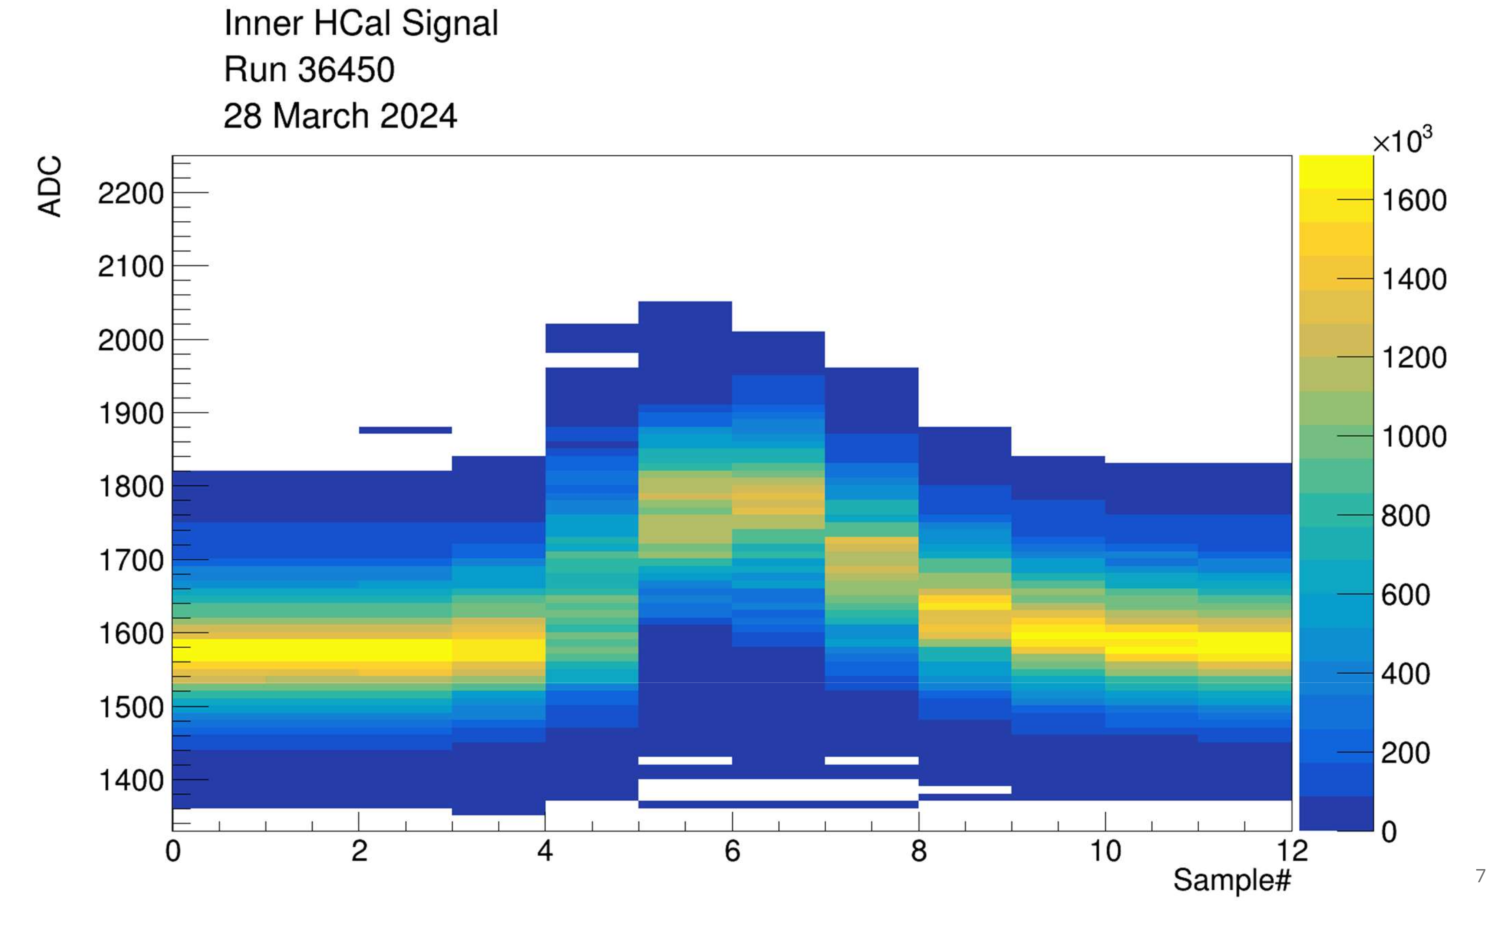
\includegraphics[width=6cm]{pulser_waveform}
				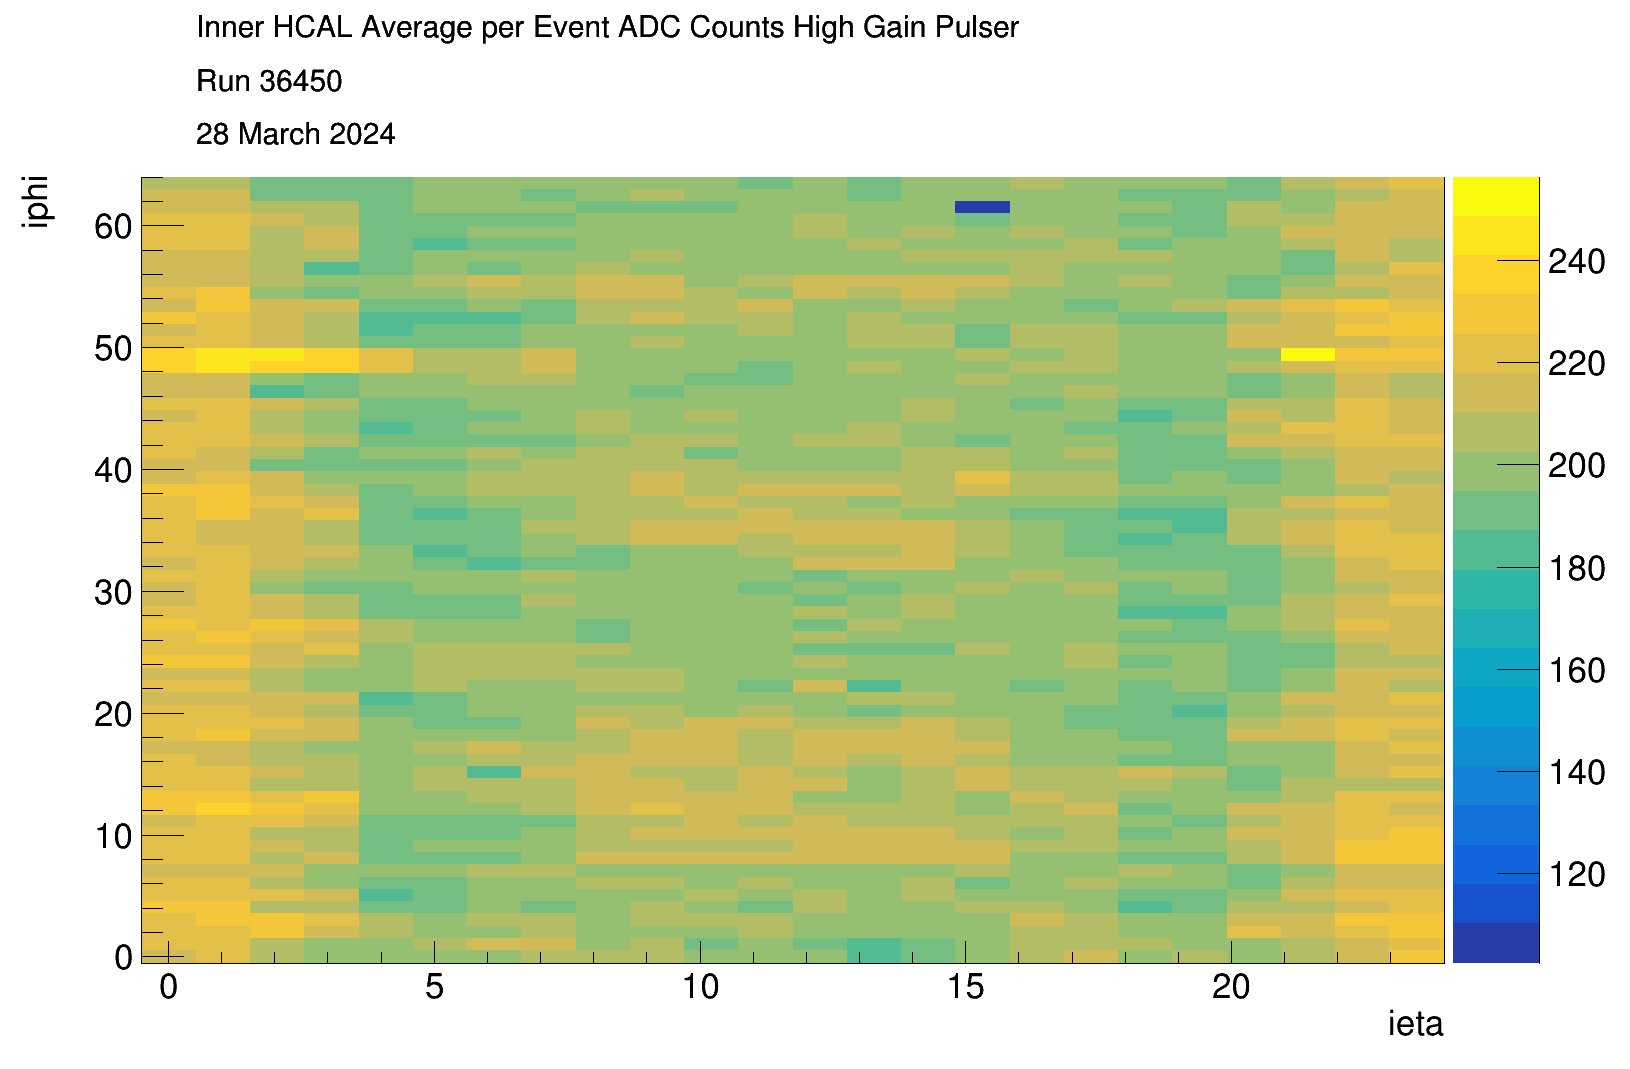
\includegraphics[width=6cm]{ihcal_pulser.png}
				\caption{Charge Injection Pulse. This system allows for direct testing of electronics without detector response}
			\end{subfigure}
			\hfill
			\begin{subfigure}[t]{0.4\textwidth}
				\includegraphics[width=6.5cm]{led_waveform}
				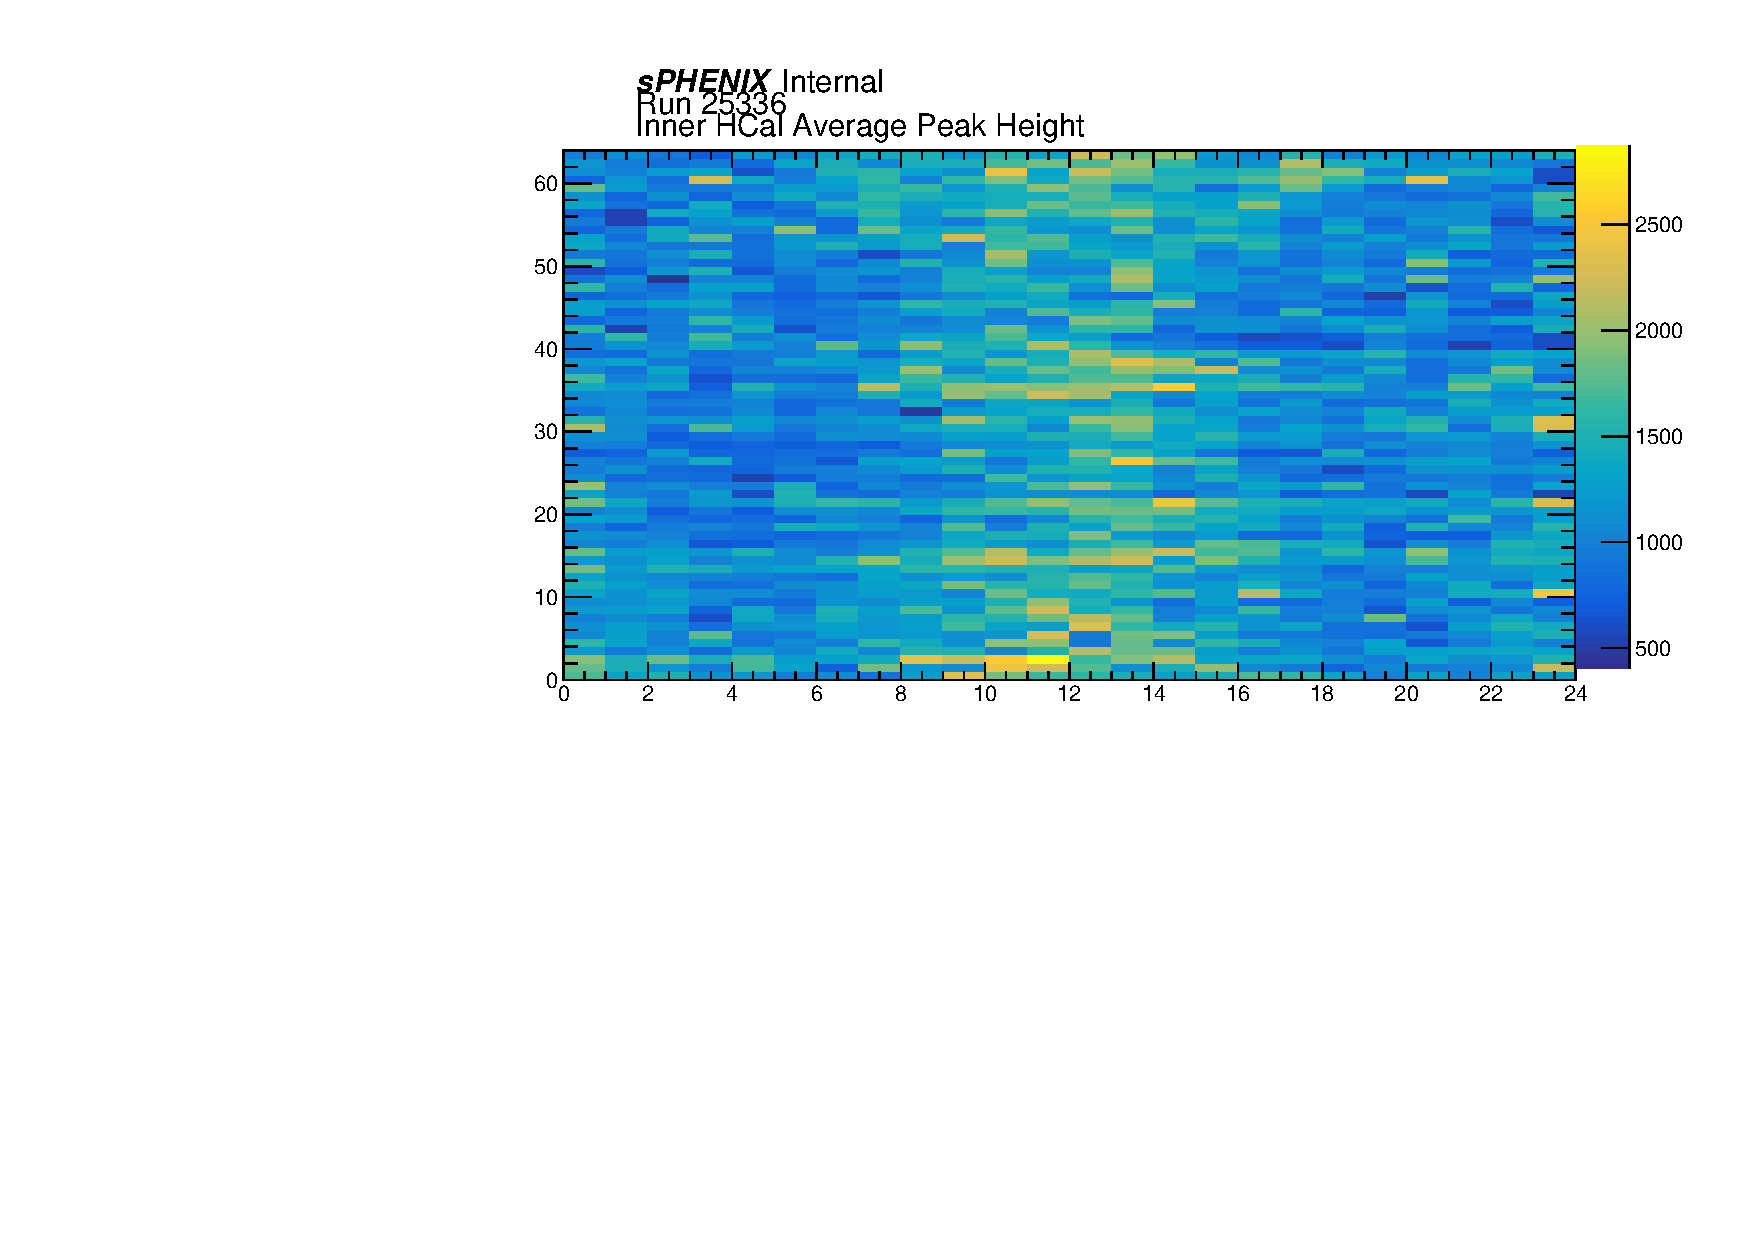
\includegraphics[width=6cm]{ihcal_led}
				\caption{LED pulse. This allows for testing of the full readback system and light response}
			\end{subfigure}
				\caption{Top: Presistence Waveform. Bottom: Energy distribution averaged across $10^{5}$ events}
			\label{fig:hcal_tests}
		\end{figure}
		\subsubsection{Calibration}
			The hadronic calorimeters were intially calibrated through use of cosmic ray muons, matching the spectra to Monte Carlo 
			generated through EcoMug and GEANT4 \cite{HCal_Calib}. 
			This calibration is updated through out the run via continued cosmic ray studies in between physics data taking in addition
			to ongoing work on in-situo calibrations using tower-slope methods \cite{tower_slope_hcal}. 
			These calibrations have yeilded an average conversion factor for the OHCal of and the IHCal of %*put ing the factor here*%
	\subsection{Electromagnetic Calorimeter}
		Moving in one layer from the hadronic calorimeter, the Electromagnetic Calorimeter (EMCal) has the same coverage in $\eta-\varphi$ space,
		but has 16 times as many towers with 96 bins in $\eta$ and 256 bins in $\varphi$. 
		The EMCal is constructed of blocks of tungsten with embedded scintilationg fibers, 
		and had inner radius $r=0.9$ m and outer radius of $r=1.16$ m.
		Similarly to the HCals, the EMCal is also equipped with a pulser and LED, although the increased number of towers and higher varaiblility 
		in response requires that different pulse widths be used for seperate sets of towers to prevent saturation and clipping on the LED pulse.
		\subsubsection{Calibration}
			The EMCal was calibrated to the $\pi^0$ mass through the $\pi^0 \rightarrow \gamma \gamma$ decay channel with additional corrections
			applied via the tower slope. 
			The mean $m_{\pi^0}$ and width are used as quality assurance plots to monitor radiation damage to the EMCal on an ongoing basis.
	\subsection{Zero Degree Calorimeter}
		The Zero Degree Calorimeter (ZDC) is a small transverse energy hadron detector that positioned outside of the experiment hall, in the tunnels along the beam pipe, 18 m from the interaction point on both side.
		The ZDC is used to detect spectator neutrons to allow for the calculation of multiplicity and event geometry, making it an overlapping detector between the calorimeters and the event characterization \cite{sphenix_ZDC}. 
		In addition, the ZDC provides a good proxy for total collision rates, useful for both real time monitoring of beam conditions and 
		The sPHENIX ZDC is one of two detectors that was preserved from PHENIX, with minor repairs and upgrades to improve running.
		In pp collisions, the ZDC provides additional utility as a spin momentum detector that allows for measurment of the spin patterns of the RHIC beam through the Vernier Scan. 
		This functionality is pivotal for the development of sPHENIX's spin physics program in pp and its extensions into the continuing physics goals at the Electron Ion Collider (EIC)\cite{sphenix_ZDC}.
		For the purposes of this work, the ZDC is not utilized for either spin phyiscs or trigger capabilities and serves primiarily to help establish cross-sections for error determination. 
		While this work does not dive into the subject of spin depenendence, such topics are a natural extension and present an intresting avenue for future studies in this vien to be done with the sPHENIX Run 24 data set. 

\section{Tracking}
	The sPHENIX tracking system consits of the Silicon vertexing detectors and the gas based trackers.
	\subsection{INTT}
	\subsection{Micromegas Vertex Detector}
	The Micromegas Vertex detector (MVTX) is a silicon based vertexing detector based on a similar system at the ALICE experiment of the Large Hadron Collider (LHC). 
	\subsection{Time Projection Chamber}
	The Time Projection Chamber (TPC) 
	\subsection{TPC Outer Tracker}
	The TPC Outer Tracker (TPOT) was designed as a minimal add-on to improve tracking effeciency and resolution by providing additional track points. 
\section{Event Characterization}
	\subsection{sPhenix Event Plane Detector}
	\subsection{Minimum Bias Detector}
	The sPHENIX Minimum Bias Detector (MBD) is the other detector preserved from PHENIX, when it was called the Beam-Beam Counter (BBC). 
	This detector is situated  
\section{Triggers}
	The sPHENIX detector has a number of triggers at its disposal to allow for online event type selections for the triggered readout system: the EMCal, the HCals, the ZDC, the MBD, the sEPD and--for run 2024--the TPC.
	Starting in run 2024, available triggers are Minimum Bias 
	\section{
\chapter{Monte Carlo Simulations}
	We have some of them, there is some data from the 2 and three point energy correlator, and its important for training of our discriminator 
\chapter{Determining Backgrounds and Errors}
\part{Technicalities: The finer points of theory and computing}
\chapter{The Energy Correlator and the primary vertex}
	So the energy correlator alows a look back, I guess thats the relevant bit? 
	Point being, if the jet points back to the primary vertex, the share of the energy between the jets and the composition of those jets is directly determined by the $2 \rightarrow 2$ scattering and is thus sensitive to the parton distribution functions of the beam particles. 
	Starting from the definition of the energy correlator given in \cite{Larkoski2013}:
	\begin{equation}
		\mathcal{E}_{N} = \int \frac{\dd \Omega}{2} \int \dd \vec{n}_{12} \frac{\langle \varepsilon \left( \vec{n}_1 \right) ... \varepsilon \left(\vec{n}_2 \right)\rangle}{Q^2} \delta\left( \vec{n}_1 \cdot \vec{n}_2 - 2|\vec{n}_1|||\vec{n}_2|\cos  \theta \right)
		\label{eq:ENC}
	\end{equation}
\chapter{Jets in Vacuum and the PDF}
\section{Jet Identification Algorithms}
As discussed in chapter \ref{ch:LR}, there are a variety of jet finding algorithms that prioritize different theoretical aspects of the underlying physics while being experimentally realizable \cite{Dokshitzer1997} \cite{Atkin2015}. 

In general, a jet identification algorithm needs to be IRC safe. 
That is, the jet object needs to display invariance in the Infrared (IR) and Collinear regimes, managing real-virtual cancellation and keeping results meaningful for emission and splitting respectively. 

\chapter{So exactly how intelligent is AI}
\chapter{Proof Solving and Validation as Quality Control Mechanisms}
\part{Experimental Output: The Main Event}
\chapter{So is sPHENIX actually working?}
\chapter{Measuring the Energy Correlator}
\chapter{The Power of the ENC: $\alpha_s$ at the few GeV scale}
\label{ch:alphas}
\chapter{Event-by-Event distinguishing} 
\label{ch:qgdiscr}
\chapter{Comparison is the Theft of Joy: What does the LHC say, and how about STAR?}
\chaptermark{LHC and STAR Results}
\chapter{Entanglement and other Lofty Goals}
\part{Wrapping it all up}
\chapter{Observable prospects for Run 25 and the EIC}
\chapter{Remaining Questions}
\chapter{Implementation and application for the remaining sPHENIX data}
\chaptermark{Future Work}
\singlespacing
\printbibliography
%\bibliographystyle{apalike}
%\bibliography{thesis}
\end{document}
